\documentclass[ngerman]{scrartcl}
\usepackage{personal}
\usepackage{wrapfig}
\usepackage{graphicx}
\usepackage{subcaption}
\usepackage{listings}
\usepackage{parskip}
%\lstset{numbers=left, frame=tblr, basicstyle=\tiny, tabsize=3}
\definecolor{codegreen}{rgb}{0,0.6,0}
\definecolor{codegray}{rgb}{0.5,0.5,0.5}
\definecolor{codepurple}{rgb}{0.58,0,0.82}
\definecolor{backcolour}{rgb}{0.95,0.95,0.92}

\lstdefinestyle{mystyle}{
    backgroundcolor=\color{backcolour},   
    commentstyle=\color{codegreen},
    keywordstyle=\color{magenta},
    numberstyle=\tiny\color{codegray},
    stringstyle=\color{codepurple},
    basicstyle=\ttfamily\footnotesize,
    breakatwhitespace=false,         
    breaklines=true,                 
    captionpos=b,                    
    keepspaces=true,                 
    numbers=left,                    
    numbersep=5pt,                  
    showspaces=false,                
    showstringspaces=false,
    showtabs=false,                  
    tabsize=2
}
\lstset{style=mystyle}


\begin{document}
\begin{titlepage}
\begin{center}
    \vspace{15cm}
    \huge{Lab 2}\\
    \vspace{2cm}
    \Huge{AML}\\
    \vspace{2cm}
    \Large{Elia Faure-Rolland}\\
    \Large{Tarek Saade}\\
    \Large{Ana Martinez}\\
    \Large{Jonas Thalmeier}\\
    \vspace{1cm}
    19/05/2025
\end{center}
\vspace{3cm}
\begin{figure}[h]
    \centering
    
\includegraphics[width=.5\textwidth]{Figures/Eurecom.png}
\end{figure}
\end{titlepage}

%\newpage
%\tableofcontents
\thispagestyle{empty}
\newpage
\setcounter{page}{1}

\section{Introduction}




\section{Method 2: LSTMs for frame prediction}

As a second method, we adopted a different approach from the first. 
Initially, we visualized various samples from the dataset by sampling the audio file with a sample rate of 16k, using a mono channel, to better understand the main differences between anomalous and normal data. 
We represented the audio signals in both the time and frequency domains and highlighted the key distinctions between samples from the two groups.
\\Since the representation in the frequency domain alone did not prove meaningful for our task, we decided to proceed by applying a representation on the spectrogram \ref{fig:spectograms},
 enabling visualization of variations in both time and frequency domains. Figure \ref{fig:spectograms} shows two signals, respectively anomalous and normal. 
 We observe that the anomalous signal is characterized by higher frequencies occurring at intervals defined in the time domain, while the anomalous signal is more regular and stable.

Our method is based on dividing the signal into frames and using an LSTM model to predict the next frame. The strategy can be summarized in the following steps:
\begin{enumerate}
  \item Train an LSTM model on the training data (consisting only of normal data) to learn the normal behavior.
  \item Test the model on an evaluation set, taken from the training data, to assess its performance on unseen normal samples.
  \item Compute the prediction error to define a classification threshold \( T \).
  \item Test the model on the test set and compute the error for each sample. If the sample’s error exceeds \( T \), classify it as anomalous data.
\end{enumerate}


In particular, the spectrogram of each sample was characterized by 313 frames (in the time domain) with 128 features each (each feature corresponds to a frequency value). 
We used a sliding window to define sequences of 10 frames and built the ground truth as the next frame of the spectrogram. 
This resulted in 303 sequences for each sample, and a total of \(303 \times \text{\#input\_dimension}\) sequences for the training set.
We subsequently trained a 2-layer LSTM with an input size of 128 and a hidden size of 256 for 10 epochs, using a learning rate of \texttt{1e-3} and  abatch size of 32.

For phase \(2\), the model was evaluated on the evaluation set, and for each sample we computed the average prediction error across all 303 sequences.
Then, we calculated the overall average prediction error and variance across all samples. 

We tested different threshold values, both considering the variance and ignoring it, and observed the best performance on the test set.

Finally, we plotted the ROC curve to determine the best threshold value.

Figure \ref{fig:rocLSTM} shows the ROC curve obtained by considering all possible threshold values from the evaluation phase. The final AUC (Area Under the Curve) value was 0.9406, which represents our best result and is close to the ideal case where the True Positive Rate is 1 and the False Positive Rate is 0.

We also computed the optimal threshold value by selecting the point on the ROC curve closest to the top-left corner, which corresponds to the ideal classifier with a True Positive Rate of 1 and a False Positive Rate of 0. 
This was done by calculating the Euclidean distance between each point \((\text{FPR}, \text{TPR})\) on the curve and the point \((0, 1)\), and choosing the threshold that minimizes this distance. 
The best threshold found was approximately 0.001688, which is close to the mean prediction error observed during the evaluation phase.


As shown in Table \ref{tab:results}, setting the threshold to 0.001688 yielded strong performance metrics in terms of precision, recall, and overall F1 score.

\begin{figure}[h]
    \centering
    \includegraphics[width=.5\textwidth]{C:/Users/elyfa/OneDrive - eurecom.fr/AML/Report2/Figures/ROC\_LSTM.png}
    \caption{ROC curve for the LSTM model}
    \label{fig:rocLSTM}
\end{figure}

\begin{figure}[h]
    \centering
    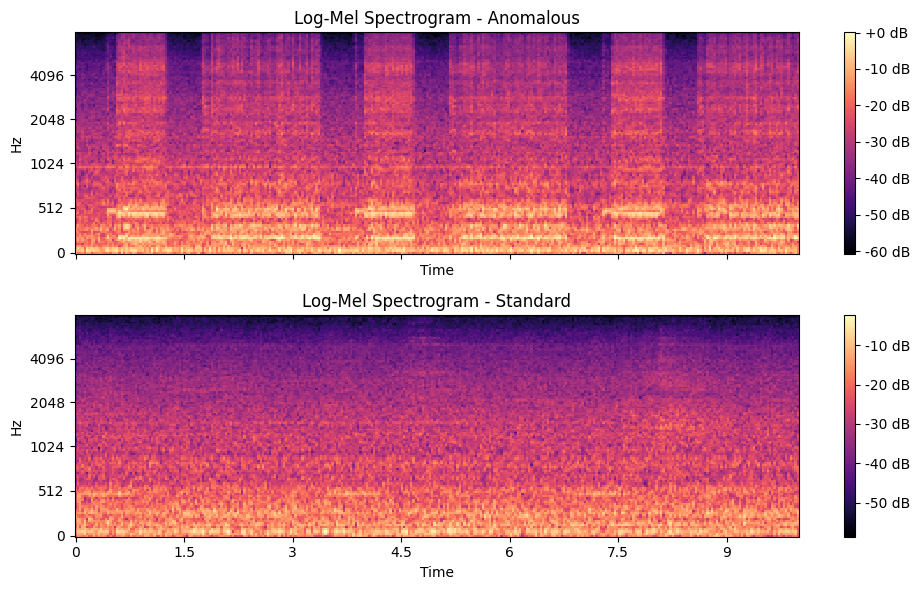
\includegraphics[width=.5\textwidth]{C:/Users/elyfa/OneDrive - eurecom.fr/AML/Report2/Figures/spectograms.png}
    \caption{Spectrograms for Anomalous (top) and Normal samples (bottom). As we can observe normal samples are characterized by more stability and lower frequencies.}
    \label{fig:spectograms}
\end{figure}


\begin{table}[h]
    \centering
    \begin{tabular}{|c|c|c|c|}
        \hline
        Class & Precision & Recall & F1-score \\
        \hline
        normal  & 0.76  & 0.90   & 0.82   \\
        anomalous  & 0.96  & 0.89  & 0.92  \\
        \hline
    \end{tabular}
    \caption{Results for LSTM classifier with threshold 0.001688.}
    \label{tab:results}
\end{table}






\section{Model Architecture}
\end{document}